
% METHODOLOGY
% •	Study area description, if any
% •	Justify certain choices of methods and datasets
% •	Be clear on what will be investigated using what metrics. For example, the research will study the uptake of solar panel installation for different provinces by comparing the number of households that have solar panel installations since 2015. 
% •	Be clear on how to validate the results and using what metrics. For example, assess the accuracy of detecting solar panels using overall accuracy, user’s accuracy, precision, etc.,
% •	Clearly describe any ground truth or reference data, e.g., how to access and how/what to collect
% •	page indication: 2 

\subsection{Study area}
%question regarding restriction of biotic dispersal?
The study area was located at two provinces in the south of Mexico, the province of Oaxaca and the province of Chiapas (Fig. \ref{fig:sa}). The dry tropical forest site was located at the area of Nizanda (16°39' N, 95°00' W), Mexican province of Oaxaca at an elevation of 90-120~m a.s.l. and the wet tropical forest was located at the area of Loma Bonita (16°01' N, 90°55'), Mexican province of Chiapas, at an elevation of 115-300~m a.s.l.. 

\begin{figure}[htbp]
\centering
\includegraphics[width=\linewidth, keepaspectratio]{Report/figures/01_studyarea3.png}
\caption{\textit{Study area.}}
\label{fig:sa}
\end{figure}

The dry tropical forest has a mean annual temperature of 27.7°C and seasonal rainfall with a mean annual precipitation of 900~mm where 90\% of the total annual rainfall occurs between May and October. It is characterized as dry tropical deciduous forest \citep{hordijkLandUseHistory2024}. The wet forest has a mean annual temperature of 24°C and a mean annual precipitation of 3000~mm with a relative dry season between February and April accounting for less than 10\% of the total annual rainfall. The vegetation varies between semi-deciduous and lowland tropical rain forest \citep{hordijkLandUseHistory2024}.

There are twenty (25~m x 25~m) research plots established in both the dry and wet tropical forest. These plots were established on a recently abandoned (0-10 months following abandonment) pasture or agricultural land by the PANTROP project in March 2020 \citep{hordijkLandUseHistory2024}. In neotropics, shifting agriculture or also known as slash and burn agriculture has been a common agricultural practice which after depletion of resources results in land abandonment \citep{jakovacRoleLanduseHistory2021}. If needed, plots were fenced off to prevent grazing. 

The extent of the study area is approximately 3~km x 2~km for the dry forest and 3~km x 5~km for the wet forest, however in order to be able to measure the characteristics of the surrounding landscape a buffer of 1~km was taken around each plot resulting in an area of approximately 5~km x 5~km for the dry forest and 7~km x 6~km for the wet forest.

\subsection{Data}

\subsubsection{Seed}
%Seed factor/variable/attribute?
To assess the seed status in the research plots, the following seed variables were identified: 1) \textbf{seed richness}: number of unique species (?ref), 2) \textbf{seed dispersal mode}: the method (biotic/abiotic) by which a seed is dispersed (?ref)  3) \textbf{seed guild}: the guild (pioneer/shadetolerant/generalist) to which a species belongs based on the characteristics of the species' resource use \citep{blondelGuildsFunctionalGroups2003}. 

To measure the seed variables in both forest sites (wet and dry), four seed traps were established in each plot. In the dry forest, the seed traps were rectangular with the dimensions of 50~cm x 50~cm and in the wet tropical forest, the seed traps were circular with the diameter of 1~m. The seed traps were positioned 6~m from the plots’ edges in each corner of the plots (Fig. \ref{fig:st}). The seeds were collected monthly for a duration of one year in 2023. The content of the four traps was combined into one sample per plot.

\begin{figure}[htbp]
\centering
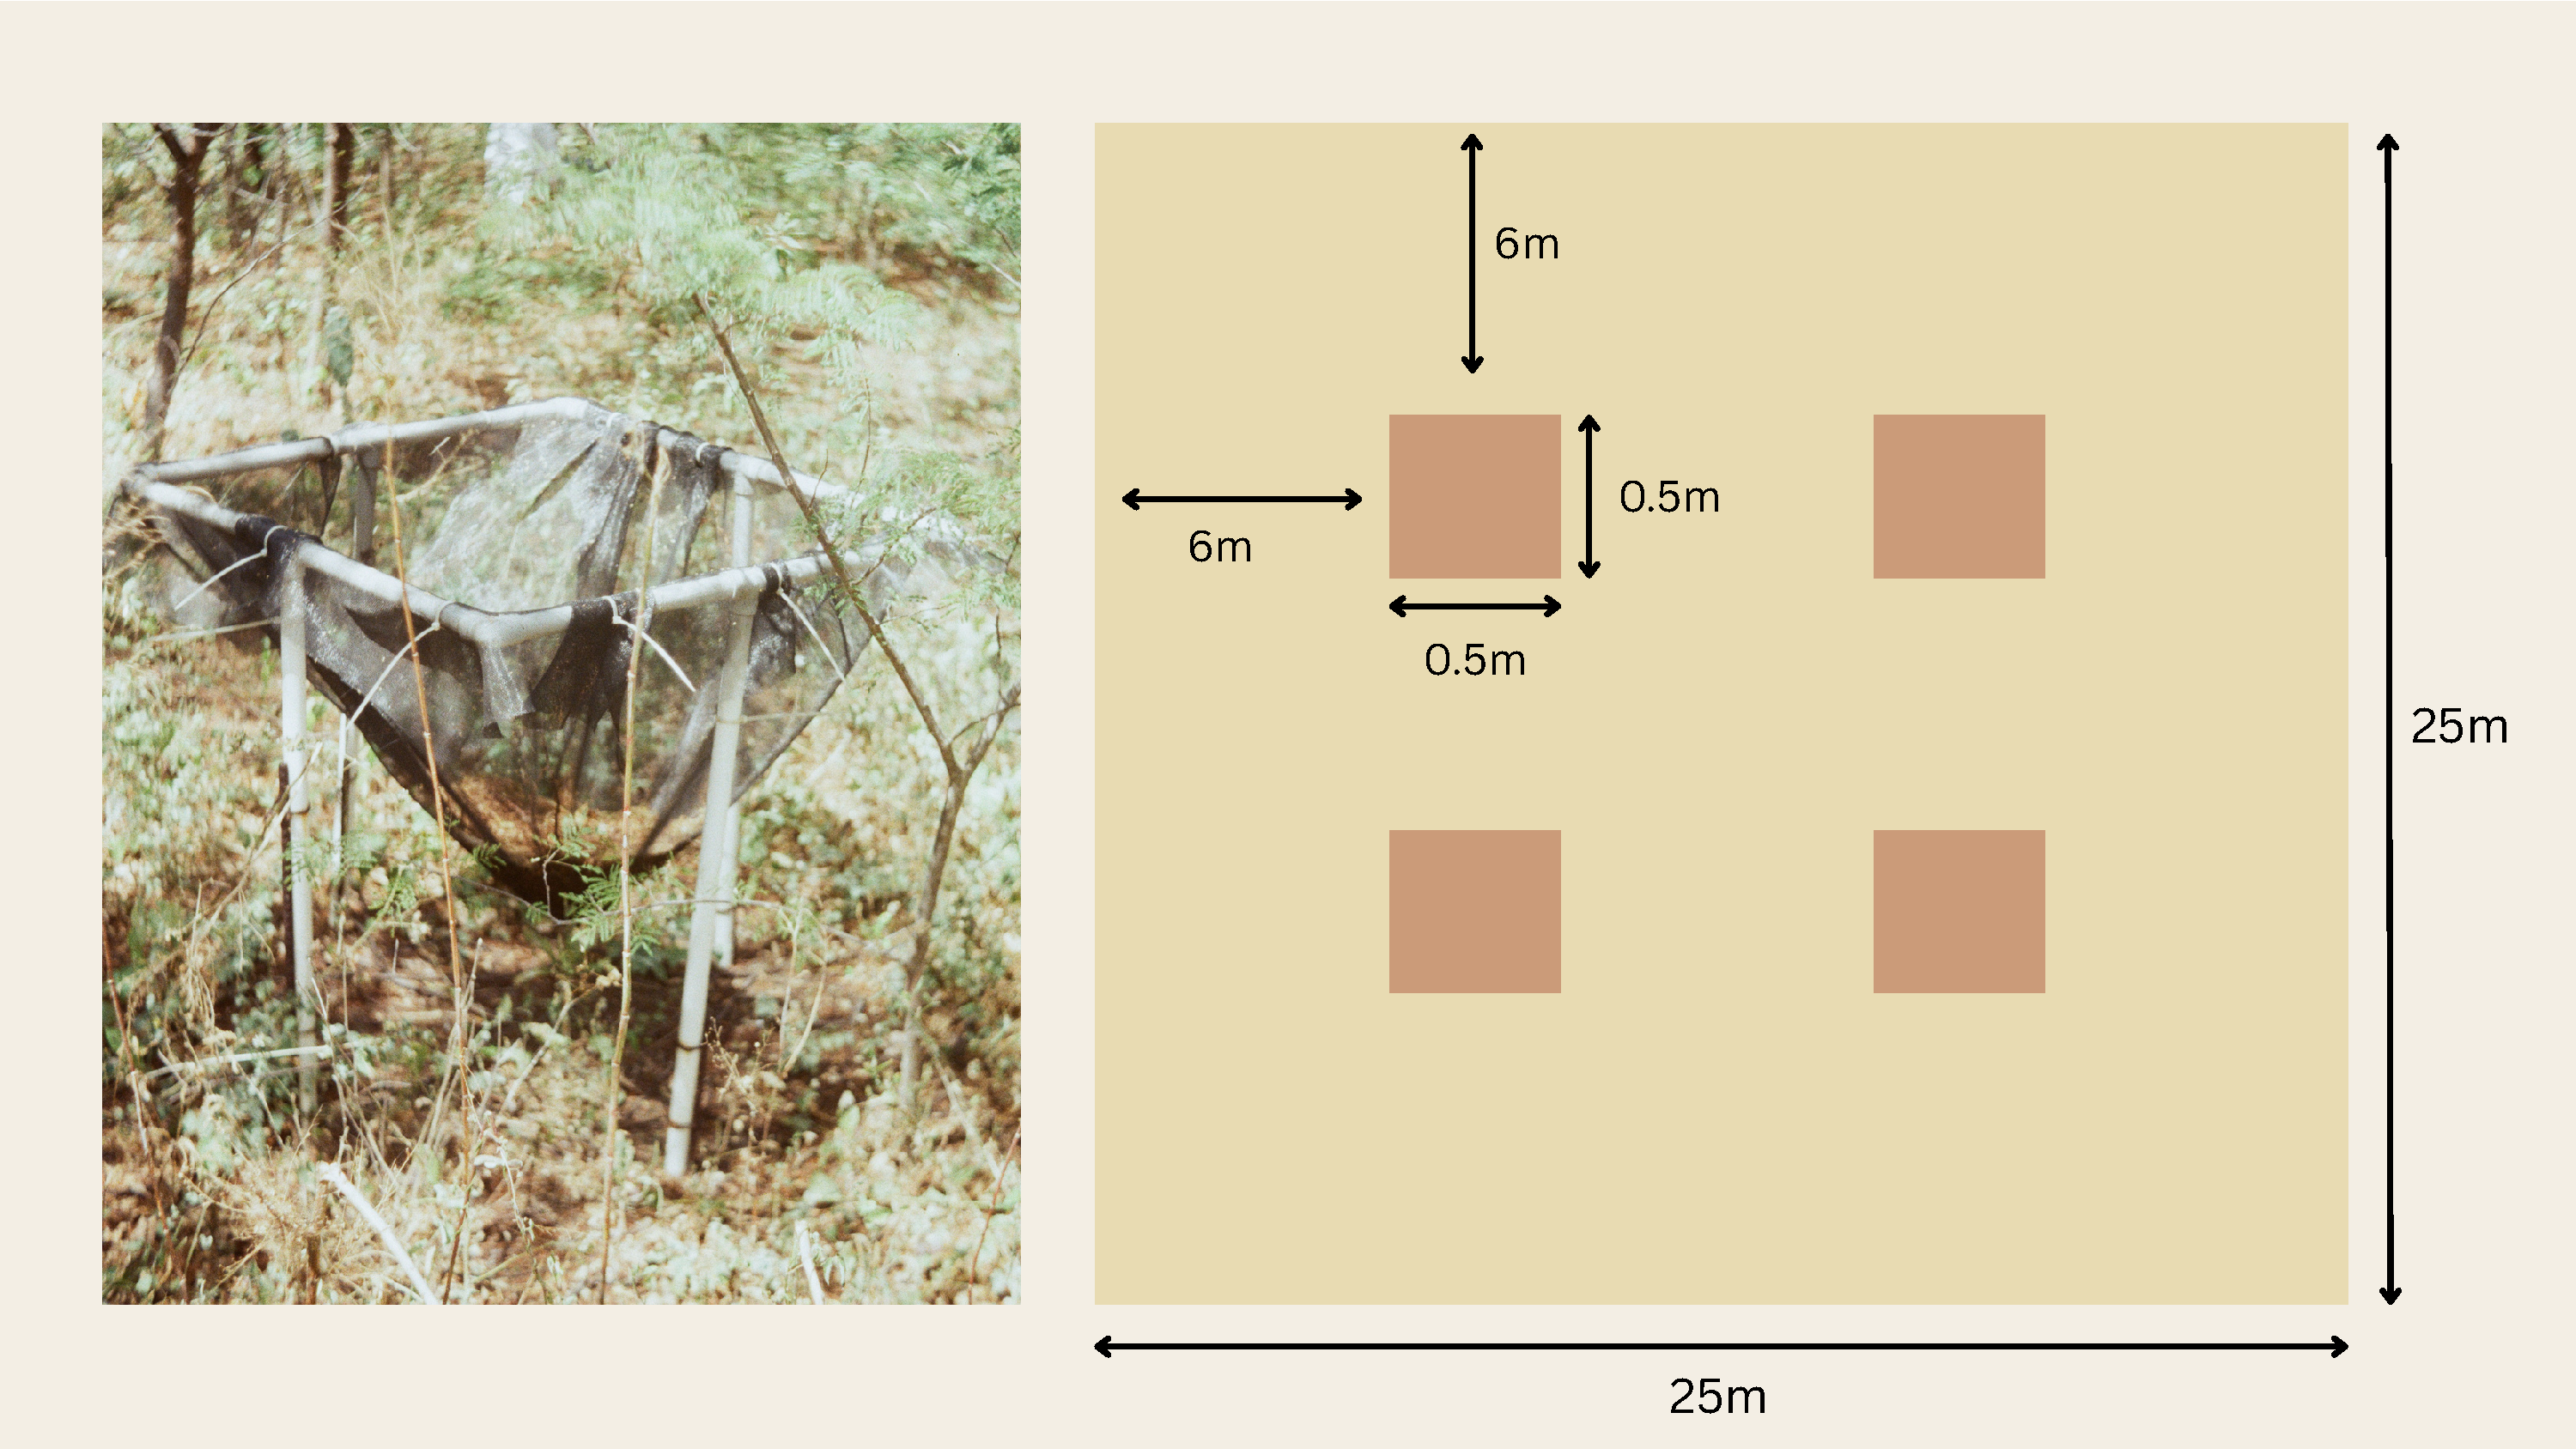
\includegraphics[width=\linewidth, keepaspectratio]{Report/figures/02_seedtraps.pdf}
\caption{\textit{Seed traps. Visualization of a seed trap on the left and the placement of seed traps in one research plot on the right. Note that in the wet tropical forest the seed traps are circular.}}
\label{fig:st}
\end{figure}

Subsequently, the collected seeds were separated into groups of unique species and identified per species. Based on literature, each species was described by their dispersal mode (biotic/abiotic) and guild (pioneer/shadetolerant/generalist). The seperation and identification of seed species was performed with a seed catalog provided by Universidad Nacional Autonóma de México (UNAM) and with the support of research assistant Marina Beatriz Hernandez Mendez, an expert in tropical wet forest seed identification, and Gerardo Luis Cervantes Jiménez, an expert in tropical dry forest seed identification. 


\subsubsection{Landscape}
%Is it a problem that the research plot itself is not cut out from the landscape evaluation?
%define research plot (regenerating forest plot?)

To  assess the forest surrounding the research plots, the following forest variables were identifined: 1) \textbf{forest age}: the number of years since last regrowth of a forest (up to a maximum of 30 years due the limit of satellite imagery), 2) \textbf{forest cover}: the percentage of forest in the surrounding landscape (ref to landscapemetrics), 3) \textbf{forest connectivity}: the mean of Euclidean nearest neighbor distances between forest patches (def of a forest patch). All forest variables were calculated within a radius of 1000km from the center of a research plot (ref to animal movement, ref to landscapemetrics).  \\

\textbf{Landsat data}\\
% Why 30 years?
% is it a poblem that the research plots are included in the landscape??
%Remote sensing techniques have become an invaluable tool for assessment of landscape. With historical field data being scarce and interview-based data being unreliable and difficult to obtain, remote sensing techniques offer a robust method for analysis of landscapes with large spatial extents \citep{decuyperContinuousMonitoringForest2022}.

In this research, images from Landsat 5 Thematic Mapper (TM), Landsat 7 Enhanced Thematic Mapper Plus (ETM+) and Landsat 8 Operational Land Imager (OLI) were used to assess the forest age based on the AVOCADO algorithm detecting disturbance and regrowth \citep{decuyperContinuousMonitoringForest2022}. The Landsat archive of the United States Geology Survey was selected due to its long temporal coverage extending back to the early 1970s \citep{kennedyBringingEcologicalView2014, finerCombatingDeforestationSatellite2018}. While Landsat spatial resolution (30~m x 30~m) is sometimes considered a limitation compared to its temporal resolution, it is not a significant constrain in this study, as it is comparable to the spatial extent of the investigated research plots (25~m x 25~m). 

The time series stack ranges from 1992 to 2022, consisting of 719 scenes (WRS-2 path/row: 20–21/49) for the dry tropical forest and 572 scenes (WRS-2 path/row: 22–23/48–49) for the wet tropical forest. The upper limit corresponds to the year before seed collection, as the aim was to assess the landscape conditions preceding seed dispersal.

Figure \ref{fig:satellite} visualizes the distribution of available Landsat satellite imagery data across the years of interest and date of a year for wet and dry forest. We can observe that in the early 2000s, there is a dip in the number of scenes available in both forest types. This is due to a failed mission of Landsat 6 Enhanced Thematic Mapper \citep{gowardHistoricalRecordLandsat2006}.

\begin{figure}[h]
\centering

% Top row
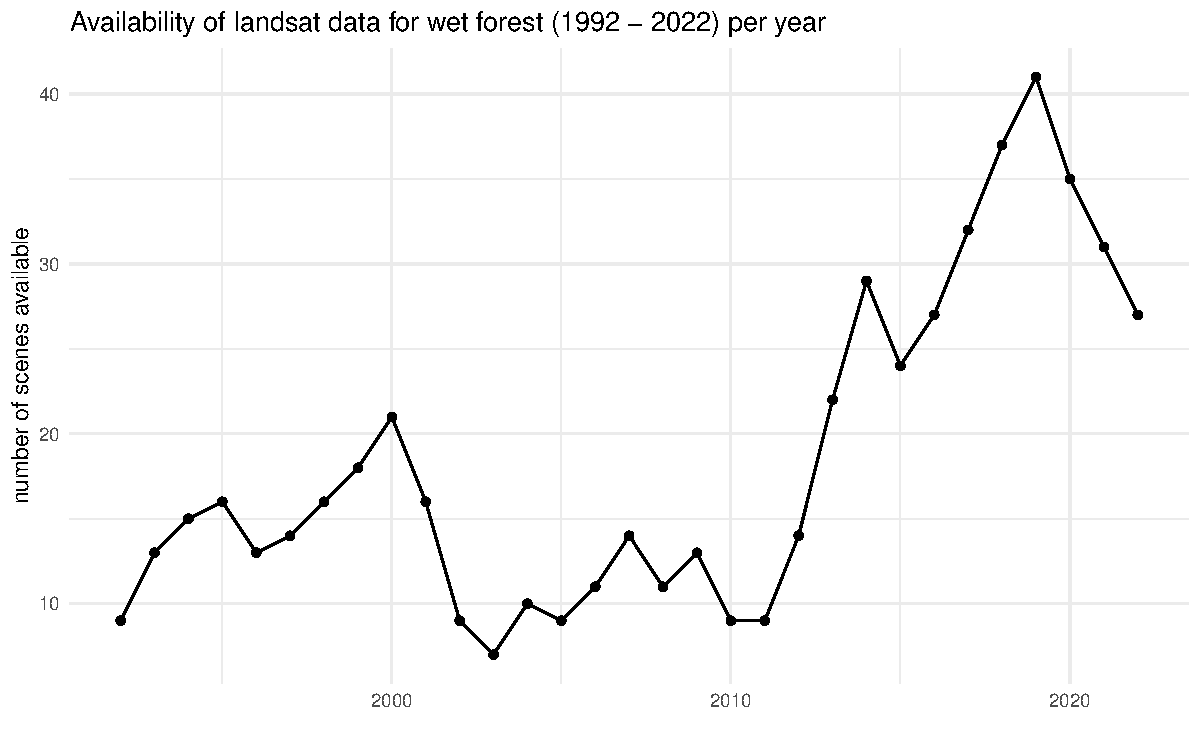
\includegraphics[width=0.48\linewidth, keepaspectratio]{Report/figures/wf_sd1.pdf}
\hspace{0.02\linewidth}
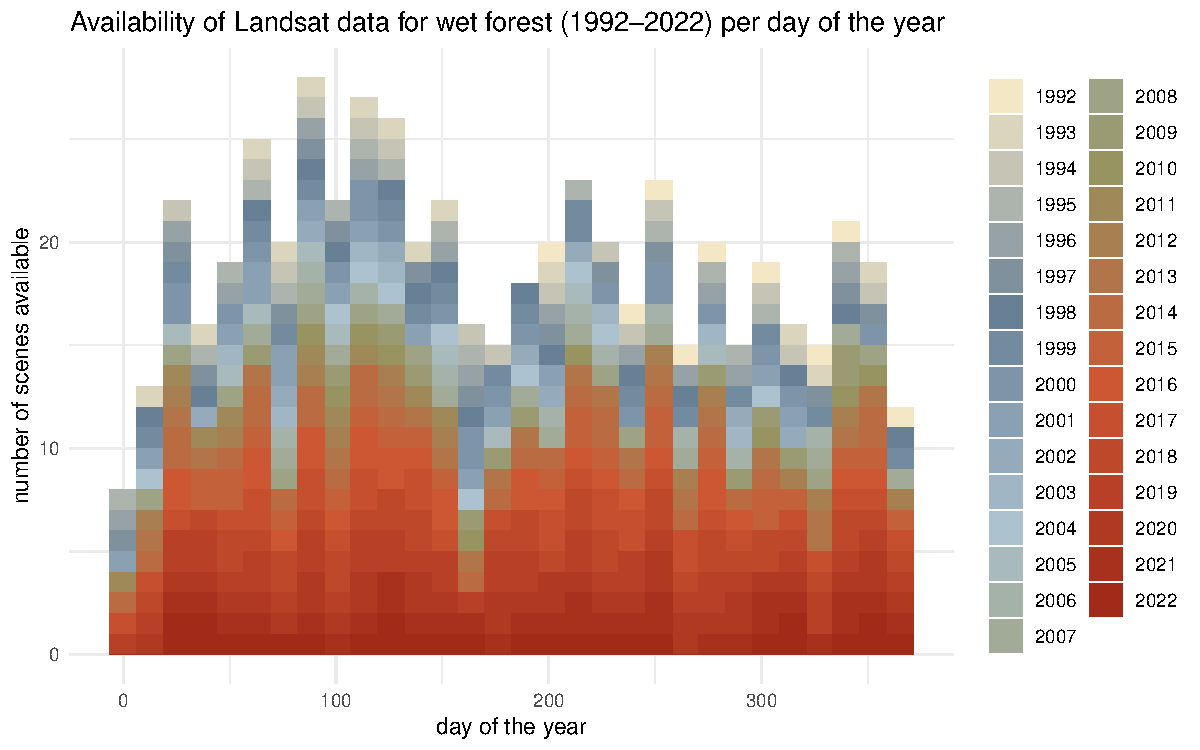
\includegraphics[width=0.48\linewidth, keepaspectratio]{Report/figures/wf_sd2.pdf}

\vspace{1cm} % Space between rows

% Bottom row
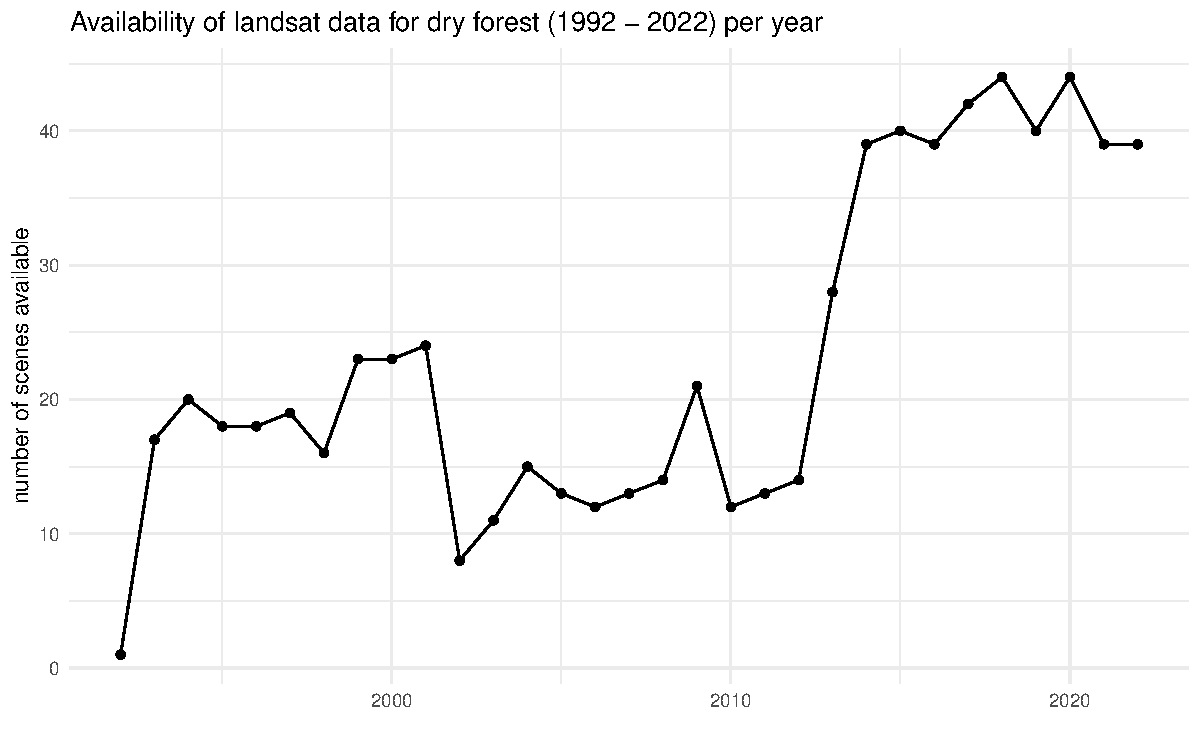
\includegraphics[width=0.48\linewidth, keepaspectratio]{Report/figures/df_sd1.pdf}
\hspace{0.02\linewidth}
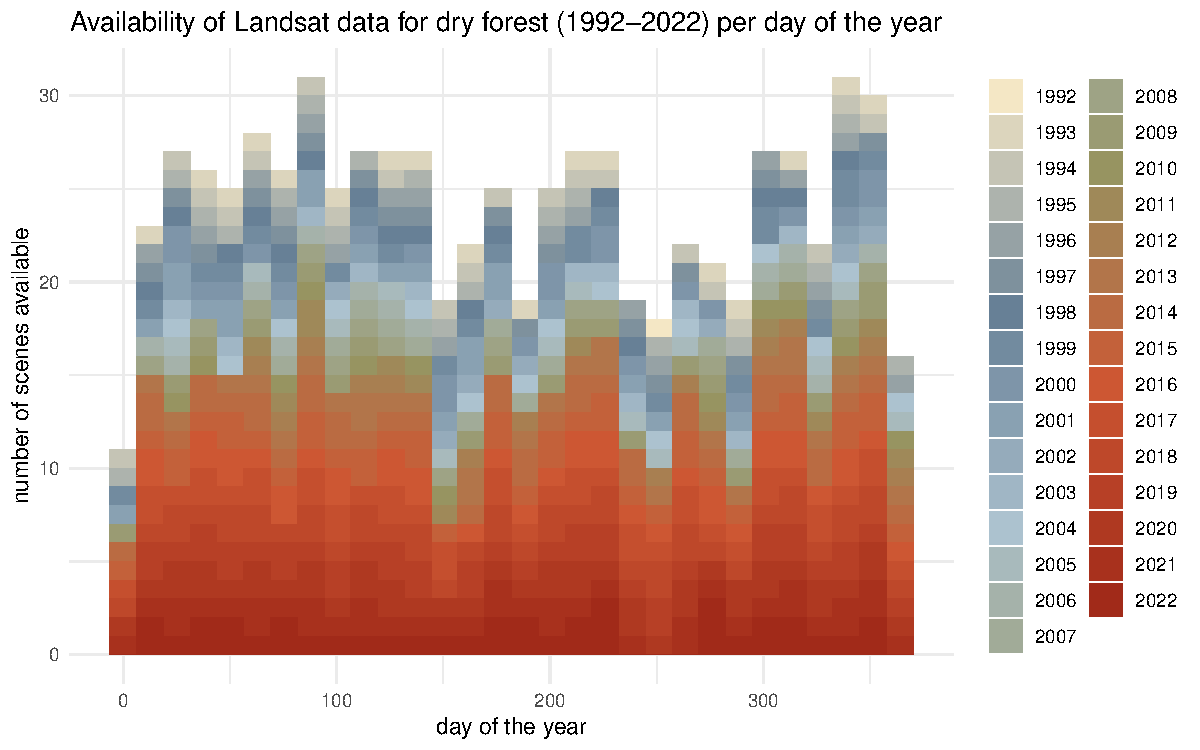
\includegraphics[width=0.48\linewidth, keepaspectratio]{Report/figures/df_sd2.pdf}

\caption{\textit{Distribution of Landsat satellite imagery availability across years of interest and date of the year. The upper row shows availability fir the wet forest whereas the lower row shows availability for the dry forest.}}
\label{fig:satellite}
\end{figure}


All atmospherically corrected Landsat Collection 2 Level-2 surface reflectance data were pre-processed and downloaded via the Google Earth Engine (GEE) platform \citep{gorelickGoogleEarthEngine2017}. Pre-processing steps included selecting scenes with less than 70\% cloud cover, clipping to the region of interest (ROI), applying cloud masking using the quality assessment band, and calculating the surface reflectance index NDMI. The Normalized Difference Moisture Index (NDMI) (Equation~\ref{eq:NDMI}), derived from Landsat's near-infrared and short-wave infrared bands, was used due to its ability to detect gradual changes and regrowth more effectively than NDVI \citep{vermotePreliminaryAnalysisPerformance2016}.

\begin{align}
\label{eq:NDMI}
NDMI = \frac{\text{NIR} - \text{SWIR}}{\text{NIR} + \text{SWIR}}
\end{align}

Satellite data were obtained following the tutorial developed by Decuyper et al. as part of their study on continuous monitoring of forest change dynamics using satellite time series. The tutorial is available online at:
\href{https://www.pucv.cl/uuaa/labgrs/proyectos/tutorial-to-the-anomaly-vegetation-change-detection-avocado}\\

\textbf{Land cover map}\\

As the aim of this research was to evaluate the forest landscape surrounding the research plots, land cover map was used to mask out all non-forest areas. European Space Agency WorldCover map from 2021 was pre-processed and downloaded via the Google Earth Engine (GEE) platform \citep{gorelickGoogleEarthEngine2017}.

\subsection{Methods}

\subsubsection{AVOCADO algorithm}
These factors will be assessed using the Anomaly Vegetation Change Detection (AVOCADO) algorithm, which is based on the R package "npphen" and with the R package "landscapemetrics" \citep{decuyperContinuousMonitoringForest2022, chavez2017npphen, hesselbarth2019landscapemetrics}. 


AVOCADO is an algorithm designed to detect forest disturbance and regrowth based on satellite imagery in a semi-automated and continuous manner \citep{decuyperContinuousMonitoringForest2022}. It utilizes all available data without requiring outlier removal. AVOCADO uses reference vegetation from a nearby pixel known to have remained undisturbed throughout the time series. This reference pixel will be selected with the help of an expert with a long-term field experience in the area. As a time series algorithm, AVOCADO analyzes more than two satellite images to detect a change. Compared to bi-temporal difference or supervised image classification methods, time series approaches offer greater precision in detecting small-scale forest changes by capturing the dynamic behavior of vegetation over time. This advantage is essential when analyzing forest change dynamics within a smallholder agricultural landscape, such as the one investigated in this research, which is often characterized by complex vegetation dynamics caused by forest degradation and shifting cultivation. Unlike many other traditional time series algorithms, AVOCADO holds an additional benefit in being able to detect more than one disturbance or regrowth. Moreover, time series methods such as temporal segmentation and trend analysis resolve this issue by applying parametric functions. These time series, however, rely on the assumption of a regular phenological cycles. Instead, AVOCADO uses the observed frequency values which enable for a greater flexibility to adapt to site specific conditions and account for natural phenological variability \citep{decuyperContinuousMonitoringForest2022}. Due to these traits, AVOCADO is a suitable algorithm for detection of forest age, cover, and connectivity as it continuously and flexibly monitors vegetation dynamics over time and detects multiple disturbances and regrowth events in complex, smallholder landscapes.

\subsubsection{Landscapemetrics}
The output of the AVOCADO algorithm is a raster map with an indication of the year since the last disturbance. This map will be used for a further evaluation of the forest age, forest cover, and forest connectivity using the landscapemetric or the lconnect package in R \citep{mestreLconnectPackageVersatile2023, hesselbarthLandscapemetricsOpensourceTool2019}. Additionally, a land cover map will be used to verify non-forest areas. The output of this section will be a table.

\subsection{Statistical analysis}
To investigate how seed richness, evenness and seed dipersal mode are affected by forest age, cover and connectivity, a Linear Mixed Model (LMM) will be performed. Linear mixed model is used to account for the nonindependent nature of the field plots, which occur in the same area and likely share highly similar environmental conditions. These field plots will be recognized as random effects of the model. Moreover, the forest landscape attributes (forest age, forest cover and forest connectivity) will be recognized as fixed effects (independent variables), whereas the seed attributes (seed richness, seed evenness and seed dispersal) will be recognized as the dependent variables. Nine models will be performed, each examining a relationship between one independent variable (forest age, forest cover, forest connectivity)  and one dependent variable (seed richness, seed evenness, seed dispersal). The model will be evaluated using $r^2$, RMSE and AIC. Additionally, p-values will be used to evaluate the significance of the predictor variables with a 0.05 level of significance. K-fold cross validation method will be applied to assess model's predictive performance. The data will be divided into k folds (the exact number of folds is to be determined), where each fold will be used for validation and the remainder of the data will serve for model's training. RMSE will be calculated for each fold and the average will be reported to assess the overall predictive performance.
To answer the research questions, the $r^2$ will be discussed to determine how much variance in predicted variable is explained by the predictor variable, while p-values will assess the statistical significance of the relationships. Finally, RMSE willl be used to evaluate the real-world applicability of the model's predictions.  

The evaluation will be performed in R software \citep{R}.

 